\documentclass{article}
\usepackage{amsmath, amssymb,amsfonts,mdframed, tikz}
\usepackage[ruled,linesnumbered]{algorithm2e}
\usetikzlibrary{shapes,arrows,calc,positioning,backgrounds}
\title{Algorithms \& Complexity: Lecture 11: Divide and Conquer}

\author{Sam Barrett}

\newmdtheoremenv{lemma}{Lemma}
\newmdtheoremenv{definition}{Definition}
\newmdtheoremenv{theorem}{Theorem}
\newmdtheoremenv{problem}{Problem}
\newmdtheoremenv{example}{Example}

\begin{document}
\maketitle

\paragraph{Divide and conquer} is a very natural and useful algorithmic technique.

It breaks a problem down in to smaller subproblems which can be solved recursively and recombined into a final solution.

Abstractly they can be thought as following the steps:

\begin{enumerate}
  \item Divide

        decompose the problem into smaller subproblems
  \item Conquer

        Solve the smaller subproblems, usually done recursively
  \item Combine

        Recombine the solutions to the subproblems into the final solution we return.
\end{enumerate}



\section{MergeSort algorithm}

\begin{problem}(MergeSort)
Given a list of $n$ numbers, we want to sort them in ascending order.
\end{problem}

As specified earlier, we must first divide the problem into smaller problems.

We will start by dividing in two (as it is the most trivial way)

\begin{center}
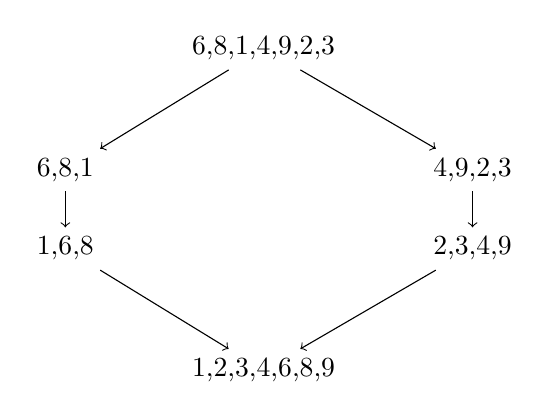
\begin{tikzpicture}
  \node (A) {6,8,1,4,9,2,3};

  \node [below left = of A](B) {6,8,1};
  \node [below of = B] (D) {1,6,8};

  \node [below right = of A] (C) {4,9,2,3};
  \node [below of=C] (E) {2,3,4,9};

  \node [below left= of E] (F) {1,2,3,4,6,8,9};


  \draw [->] (A) -- (B) ;
  \draw [->] (A) -- (C) ;
  \draw [->] (B) -- (D) ;
  \draw [->] (C) -- (E) ;
  \draw [->] (E) -- (F) ;
  \draw [->] (D) -- (F) ;
\end{tikzpicture}
\end{center}

Above you can see a very naive approach to merge sort. We split the initial problem in half, sort the halves and recombine.

Recombination in this example is done as follows:

\begin{enumerate}
  \item Initialise pointers $p_{1},p_{2}$ at the start of both sub-arrays
  \item If $A_{1}[p_{1}] < A_{2}[p_{2}]$  then append $A_{1}[p_{1}] $ to the return array and move the $p_{1}$ to the right, otherwise add $A_{2}[p_{2}] $ and move $p_2$ to the right
  \item repeat until both sub-arrays are empty (pointers cannot move to the right)
\end{enumerate}

A more formal definition for merge sort is:

\begin{algorithm}
  \caption{MergeSort($A$)}

  Divide the given list $A$ on $n$ numbers into two lists $B$ and $C$ of equal size

  Let $B'= \texttt{MERGESORT(B)} $ and $B' = \{b_{1}< b_{2}< \ldots < b_{n/2}\}$

  Let $C'= \texttt{MERGESORT(C)} $ and $C' = \{c_{1}< c_{2}< \ldots < c_{n/2}\}$

  Initialise $i=1, j=1,k=1$

  Initialise $D$ to be an empty array

  \While{$i\neq n/2 \cap j \neq n/2$}{
    \uIf{$b_{i} < c_{j}$}{
      Set $d_{k} = b_{i}$

      $k,i ++$
    }\Else{
      Set $d_{k} = c_{j}$

      $k,j ++$
    }
  }

  If one of the lists becomes empty, append the remainder of the other list to $D$

  \Return{D}



\end{algorithm}

Clearly this algorithm does not simply divide the array once, it will divide recursively until the arrays are a single element in length, relying on the recombination process to actually sort the array.

The time needed to recombine $B'$ and $C'$ to obtain $D$ is $O(n)$.

Therefore, the recurrence is $T(n) \leq 2\cdot T(n/2) + O(n)$.

We can show (but won't) that $T(n) = O(n\log n)$ satisfied this recurrence.

\section{Solving recurrences}

At the end of the merge sort section we saw that we formulated a recurrence to describe the complexity of our divide and conquer algorithms.

There are two main methods for solving these recurrences.


\subsection{Method 1: \textit{Unrolling} the recurrence}

In this method we \textit{open up} the recurrence step-by-step. It does not require any knowledge of the final result of the process.

We start by writing our recurrence for some constant value $c$:

\[
  T(n) \leq 2 \cdot T(n/2) + cn, \forall n > 2
\]

Base Case: $T(2) \leq c$

\begin{center}
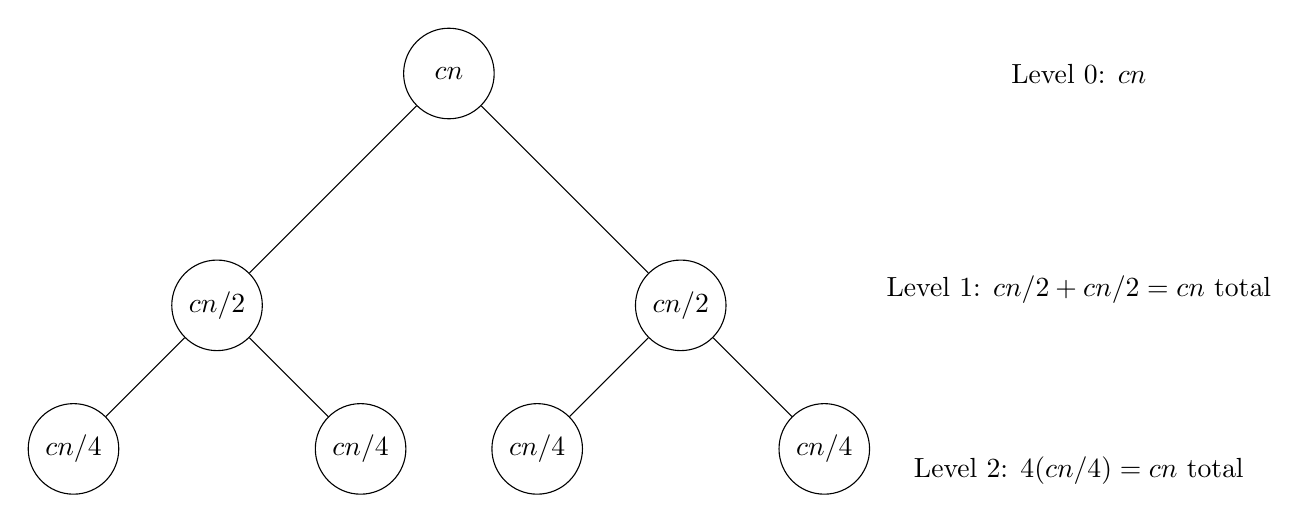
\begin{tikzpicture}
  \node [draw, circle, minimum size =1.15cm] at (-2,0) (A) {$cn$};

  \node [draw, circle, below left= 3cm of A, minimum size =1.15cm] (B1) {$cn/2$};
  \node [draw, circle, below right =3cm  of A, minimum size =1.15cm] (B2) {$cn/2$};

  \node [draw, circle, below left= of B1, minimum size =1.15cm] (C11) {$cn/4$};
  \node [draw, circle, below right = of B1, minimum size =1.15cm] (C12) {$cn/4$};

  \node [draw, circle, below left= of B2, minimum size =1.15cm] (C21) {$cn/4$};
  \node [draw, circle, below right = of B2, minimum size =1.15cm] (C22) {$cn/4$};

  \node at (6,0) (l1) {Level 0: $cn$};
  \node [below= 2.2cm of l1] (l2) {Level 1: $cn/2 + cn/2 = cn$ total };
  \node [below= 1.7cm of l2] (l333) {Level 2: $4(cn/4) = cn$ total};

  \draw (A) -- (B1);
  \draw (A) -- (B2);

  \draw (B1) -- (C11);
  \draw (B1) -- (C12);

  \draw (B2) -- (C21);
  \draw (B2) -- (C22);

\end{tikzpicture}
\end{center}

Note that at each step/level we have exactly $cn$ running time. This is our pattern, and would continue until we reach a level in which each node is of size 2 in which case we can use our base case.

We must now sum over all levels of the recursion. We will have $\log_{2}n$ levels as our base case is that $n=2$. It will take $\log_{2} n$ splits until we reach sub-arrays of size 2.

We can therefore say that as we have $\log_{2} n$ levels and each level has $cn$ running time, that our overall running time is $cn \cdot \log_{2} n$.

We can formalise this process as follows:

\begin{enumerate}
  \item Write the recurrence explicitly for some constant $c$

        $T(n) \leq 2 \cdot T(n/2) + cn$
  \item Construct our base case

        $T(2) \leq c$

  \item Analyse the first few levels

        Level 0 takes $cn$ time, and delegates two recursive calls of size $n/2$

        Level 1 takes $c(n/2) + c(n/2)$ time and delegates four recursive calls of size $n/4$

  \item Identify a pattern

        The number of subproblems doubles at each level

        The size of each subproblem halves at each level

        Level $j$ has $2^{j}$ subproblems each having size $n/2^{j}$

        So level $j$ takes a total of $2^{j}\cdot (c\cdot (n/2^{j})) = cn$ time and delegates some tasks to the next level

  \item Sum up over all levels of the recursion

        There are $O(\log_{2}n)$ levels of the recursion

        Each level requires a running time of $cn$

        $T(n) = cn\cdot \log_{2}(n) = O(n\cdot
        log_{2}n)$
\end{enumerate}




\subsection{Verifying by substitution in the recurrence}

This works well if you already have a \textit{guess} for the running time. You can then check by induction whether your guess satisfies the recurrence.

\begin{itemize}
  \item \textbf{Base Case:} $n=2$

        $T(2) \leq c \leq cn \log n$

  \item \textbf{Inductive Hypothesis}

        For each $2\leq m \leq n$ we have $T(m) \leq cm \cdot \log m$


  \item \textbf{Inductive step}

        \begin{align*}
          T(n) &\leq 2T(n/2) + cn && \text{(by the recurrence)}\\
                &\leq 2c\cdot (n/2) \cdot \log(n/2) + cn && \text{(by inductive hypothesis since $n/2 < n$)}\\
                &= cn(\log n -1) + cn  && \text{(since $\log(n/2) = \log n -1$)}\\
                &= cn\cdot \log n &&
        \end{align*}
\end{itemize}

\textbf{NOTE: we have here verified that $T(n) = cn \cdot \log n$ is \underline{one} possible solution for this recurrence, unlike the unrolling method, this method may lead to verifying that a much higher running time is correct.}

\end{document}

